%%%%%%%%%%%%%%%%%%%%%%%%%%%%%%%%%%%%%%%%%
% Wenneker Assignment
% LaTeX Template
% Version 2.0 (12/1/2019)
%
% This template originates from:
% http://www.LaTeXTemplates.com
%
% Authors:
% Vel (vel@LaTeXTemplates.com)
% Frits Wenneker
%
% License:
% CC BY-NC-SA 3.0 (http://creativecommons.org/licenses/by-nc-sa/3.0/)
% 
%%%%%%%%%%%%%%%%%%%%%%%%%%%%%%%%%%%%%%%%%

%----------------------------------------------------------------------------------------
%	PACKAGES AND OTHER DOCUMENT CONFIGURATIONS
%----------------------------------------------------------------------------------------

\documentclass[11pt]{scrartcl} % Font size

\usepackage{graphicx} % for including images
\usepackage{subcaption} % for creating subfigures
\usepackage{color}




%%%%%%%%%%%%%%%%%%%%%%%%%%%%%%%%%%%%%%%%%
% Wenneker Assignment
% Structure Specification File
% Version 2.0 (12/1/2019)
%
% This template originates from:
% http://www.LaTeXTemplates.com
%
% Authors:
% Vel (vel@LaTeXTemplates.com)
% Frits Wenneker
%
% License:
% CC BY-NC-SA 3.0 (http://creativecommons.org/licenses/by-nc-sa/3.0/)
% 
%%%%%%%%%%%%%%%%%%%%%%%%%%%%%%%%%%%%%%%%%

%----------------------------------------------------------------------------------------
%	PACKAGES AND OTHER DOCUMENT CONFIGURATIONS
%----------------------------------------------------------------------------------------

\usepackage{amsmath, amsfonts, amsthm} % Math packages

\usepackage{listings} % Code listings, with syntax highlighting

\usepackage[english]{babel} % English language hyphenation

\usepackage{graphicx} % Required for inserting images
\graphicspath{{Figures/}{./}} % Specifies where to look for included images (trailing slash required)

\usepackage{booktabs} % Required for better horizontal rules in tables

\numberwithin{equation}{section} % Number equations within sections (i.e. 1.1, 1.2, 2.1, 2.2 instead of 1, 2, 3, 4)
\numberwithin{figure}{section} % Number figures within sections (i.e. 1.1, 1.2, 2.1, 2.2 instead of 1, 2, 3, 4)
\numberwithin{table}{section} % Number tables within sections (i.e. 1.1, 1.2, 2.1, 2.2 instead of 1, 2, 3, 4)

\setlength\parindent{0pt} % Removes all indentation from paragraphs

\usepackage{enumitem} % Required for list customisation
\setlist{noitemsep} % No spacing between list items

%----------------------------------------------------------------------------------------
%	DOCUMENT MARGINS
%----------------------------------------------------------------------------------------

\usepackage{geometry} % Required for adjusting page dimensions and margins

\geometry{
	paper=a4paper, % Paper size, change to letterpaper for US letter size
	top=2.5cm, % Top margin
	bottom=3cm, % Bottom margin
	left=3cm, % Left margin
	right=3cm, % Right margin
	headheight=0.75cm, % Header height
	footskip=1.5cm, % Space from the bottom margin to the baseline of the footer
	headsep=0.75cm, % Space from the top margin to the baseline of the header
	%showframe, % Uncomment to show how the type block is set on the page
}

%----------------------------------------------------------------------------------------
%	FONTS
%----------------------------------------------------------------------------------------

\usepackage[utf8]{inputenc} % Required for inputting international characters
\usepackage[T1]{fontenc} % Use 8-bit encoding

\usepackage{fourier} % Use the Adobe Utopia font for the document

%----------------------------------------------------------------------------------------
%	SECTION TITLES
%----------------------------------------------------------------------------------------

\usepackage{sectsty} % Allows customising section commands

\sectionfont{\vspace{6pt}\centering\normalfont\scshape} % \section{} styling
\subsectionfont{\normalfont\bfseries} % \subsection{} styling
\subsubsectionfont{\normalfont\itshape} % \subsubsection{} styling
\paragraphfont{\normalfont\scshape} % \paragraph{} styling

%----------------------------------------------------------------------------------------
%	HEADERS AND FOOTERS
%----------------------------------------------------------------------------------------

\usepackage{scrlayer-scrpage} % Required for customising headers and footers

\ohead*{} % Right header
\ihead*{} % Left header
\chead*{} % Centre header

\ofoot*{} % Right footer
\ifoot*{} % Left footer
\cfoot*{\pagemark} % Centre footer
 % Include the file specifying the document structure and custom commands

%----------------------------------------------------------------------------------------
%	TITLE SECTION
%----------------------------------------------------------------------------------------

\title{	
	\normalfont\normalsize
	\textsc{}\\ % Your university, school and/or department name(s)
	\vspace{25pt} % Whitespace
	\rule{\linewidth}{0.5pt}\\ % Thin top horizontal rule
	\vspace{20pt} % Whitespace
	{\huge Automating FEM solution database generation and neural network learning for unidimensional mechanical problems}\\ % The assignment title
	\vspace{12pt} % Whitespace
	\rule{\linewidth}{2pt}\\ % Thick bottom horizontal rule
	\vspace{12pt} % Whitespace
}

\author{\Large Leopoldo Agorio, Mauricio Vanzulli, Bruno Bazzano, Jorge Perez Zerpa} % Your name

\date{\normalsize\today} % Today's date (\today) or a custom date

\begin{document}

\maketitle % Print the title

%----------------------------------------------------------------------------------------
%	FIGURE EXAMPLE
%----------------------------------------------------------------------------------------

\begin{abstract}
	This project explores the use of a neural network to solve unidimensional mechanical problems more quickly than the finite element method (FEM). We developed a pipeline for generating a database of FEM solutions to compression/extension problems and used it to train a neural network. We present the results of our experiments, including training and test loss, and compare our model to the FEM. Our approach has the potential to significantly improve the efficiency of solving mechanical problems, with broader implications for the engineering design process.
\end{abstract}
\section{Introduction}
The objective of this project is to develop a surrogate model for unidimensional mechanical problems that is faster than the finite element method (FEM). To achieve this, we trained a neural network using a dataset of FEM solutions to compression/extension mechanical problems. The ultimate goal is to apply this approach to develop state-of-the-art surrogate models for biological tissues. In this project, we used a FEM solver repeatedly to generate a large dataset of results, which was used to train the neural network. The neural network was designed to learn from the FEM solutions and solve similar mechanical problems more quickly.

This documentation report will describe the methodology used to develop the neural network, the performance of the model compared to the FEM, and potential future directions for this project. By developing a faster surrogate model, this project's approach has the potential to significantly improve the efficiency of solving unidimensional mechanical problems, with broader implications for the engineering design process.

\section{Methodology}
In this section, we describe the pipeline we developed to generate the dataset of FEM solutions and train the neural network. We used a uniaxial model with the ONSAS.m FEM solver, which we automated with a bash script. The resulting dataset was preprocessed and used to train a multi-layer perceptron (MLP) implemented in PyTorch.

\subsection{Uniaxial Model}
Our model consisted of a uniaxial mechanical problem in which a load was applied to a bar, causing it to deform. We used the ONSAS.m FEM solver to simulate the deformation and generate a dataset of solutions. The uniaxial model was chosen for its simplicity and as a starting point for more complex models.

The simulated uniaxial problem can be seen in Figure \ref{fig:uniaxial_model}. Loads are applied to the bar at the left and right ends, causing it to deform. The bar is constrained to move only in the x-direction, so the deformation is uniaxial ...

%placeholder two images side by side for the uniaxial model
\begin{figure}[h]
	\centering
	\begin{subfigure}[b]{0.48\textwidth}
	\def\svgwidth{\textwidth}
	\input{Figures/Example1.pdf_tex}
	\caption{Reference configuration sketch.}
	%\label{fig:image1}
	\end{subfigure}
	\hfill
	\begin{subfigure}[b]{0.48\textwidth}
	\centering
		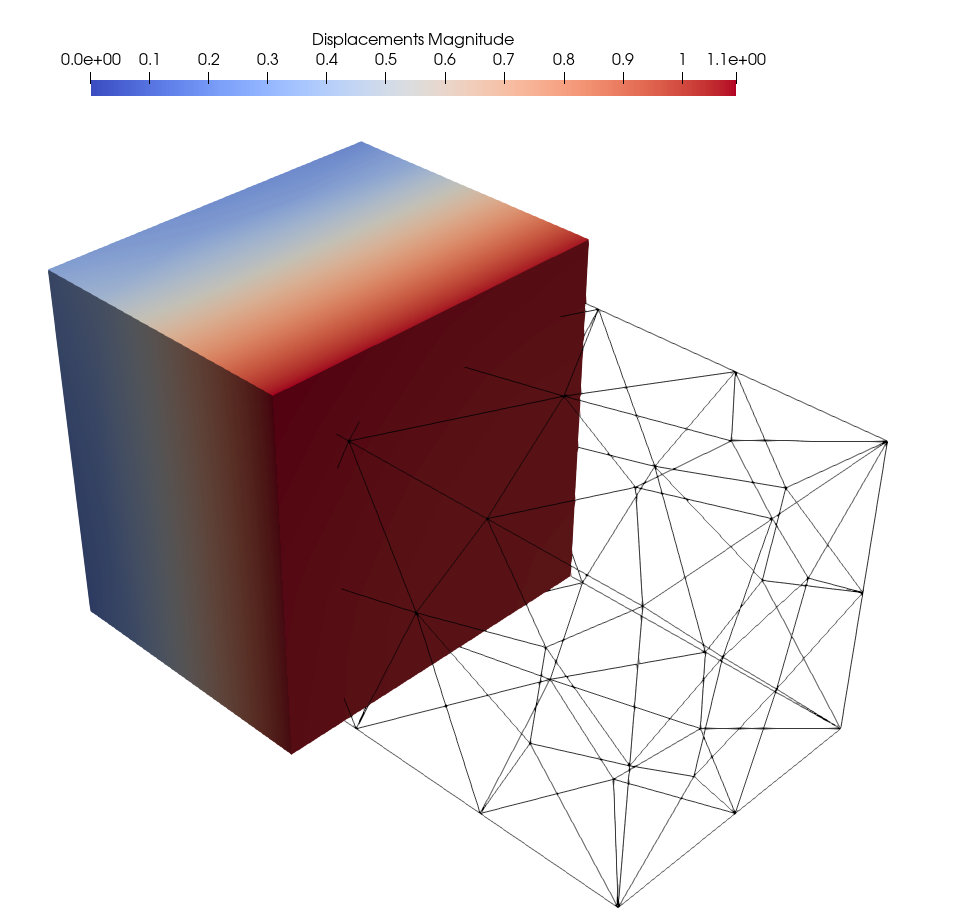
\includegraphics[width=\textwidth]{Figures/Example1.png}
	\caption{System with an applied load.}
	%\label{fig:image2}
	\end{subfigure}
	\caption{Uniaxial problem simulated and solved in ONSAS.m.}
	\label{fig:uniaxial_model}
\end{figure}


\subsection{Composed Cantilever Model}
The uniaxial model was extended to a composed cantilever model, which consisted of a prism with a second prism attached to one end. The prism was constrained to move only in the x-direction, so the deformation was uniaxial. The prism was attached to the bar at the center of its face, as shown in Figure \ref{fig:composed_cantilever_model}.
%placeholder two images side by side for the composed cantilever model
\begin{figure}[h]
	\centering
	\begin{subfigure}[b]{0.48\textwidth}
	\def\svgwidth{\textwidth}
	\input{Figures/Example2.pdf_tex}
	\caption{Reference configuration sketch.}
	%\label{fig:image1}
	\end{subfigure}
	\hfill
	\begin{subfigure}[b]{0.48\textwidth}
	\centering
	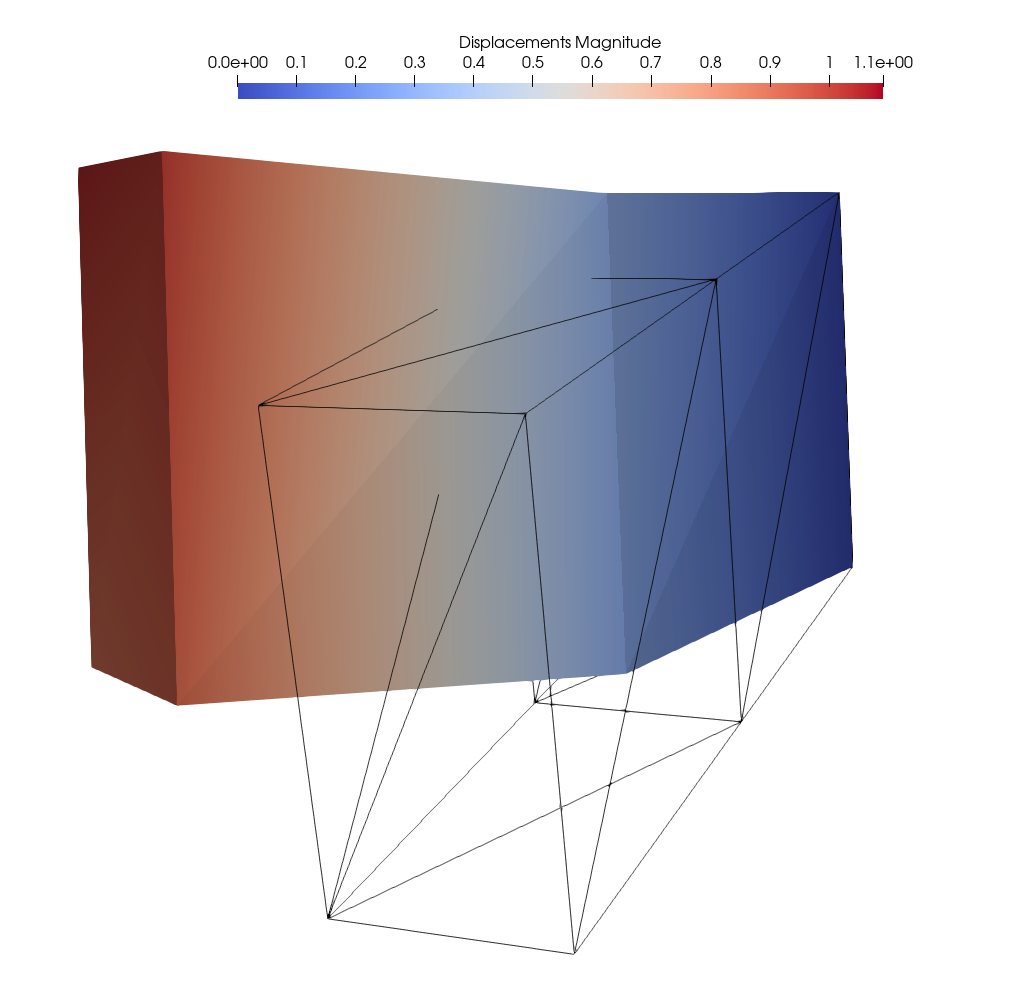
\includegraphics[width=\textwidth]{Figures/Ejemplo2.png}
	\caption{System with an applied load.}
	%\label{fig:image2}
	\end{subfigure}
	\caption{Composed cantilever problem simulated and solved in ONSAS.m.}
	\label{fig:composed_cantilever_model}
\end{figure}


\subsection{Bash Script}
To automate the FEM solver, we developed a bash script that generated the input files for the ONSAS.m solver and executed it repeatedly to generate a large dataset of solutions. The script also handled the output files, extracting the relevant data and formatting into a .csv it for further processing.

The variables sweeped by the script were the length of the bar $L_x$, the applied load $p$, and the elastic modulus of the material $E$. The output of the solver was processed to obtain the displacement of the center point of the prism's face in the three dimensions.  The script generated a total of 18900 data points, which were used to train the neural network.

For the case of the composed cantilever model, the variables sweeped were the length of the bar $L_x$, the applied load $p$, and the elastic modulus of each material $E_1$ and $E_2$. The output of the solver was processed to obtain the displacement of the center point of the prism's face in the three dimensions. The script generated a total of 13310 data points, which were used to train the neural network.

%\subsection{Preprocessing}
%The resulting dataset of FEM solutions was preprocessed to remove duplicates and normalize the input and output data. We split the dataset into training and test sets, using 80\% for training and 20\% for testing.

\subsection{Neural Network}
We implemented an MLP in PyTorch to learn from the FEM solutions and solve similar mechanical problems more quickly. The MLP had two hidden layers with 20 and 10 neurons, respectively, and used the ReLU activation function. The output layer had three neurons, corresponding to the three dimensions of the displacement of the center point of the prism's face. The optimizer was Adam with a learning rate of 0.001 and 100 epochs were used. 

In the uniaxial case we used a 50/50 split for the training and validation sets, and 200 test samples using the analytic solution. For the composed cantilever case we used 1000 samples for both the training and validation sets.

We report two different loss functions: the mean squared error (MSE) and the relative MSE. The MSE is the most common loss function for regression problems, and is defined as:
\begin{equation}
\label{eq:MSE}
MSE = \frac{1}{n} \sum_{i=1}^{n} (y_i - \hat{y}_i)^2
\end{equation}
where $y_i$ is the true value and $\hat{y}_i$ is the predicted value. The relative MSE is defined as:
\begin{equation}
\label{eq:RMSE}
RMSE = \frac{1}{n} \sum_{i=1}^{n} \frac{(y_i - \hat{y}_i)^2}{y_i}
\end{equation}
The relative MSE is more useful for comparing the performance of different models, since it is normalized by the true value.

\subsection{Analytic Solution}
To compare the performance of our neural network to the FEM, we computed the analytic solution to the uniaxial problem. The analytic solution is given by:
\begin{equation}
\label{eq:analytic_solution}
u = \frac{pL_x^3}{3E}
\end{equation}
where $u$ is the displacement of the center point of the prism's face, $p$ is the applied load, $L_x$ is the length of the bar, and $E$ is the elastic modulus of the material.

This allows us to generate a dataset of analytic solutions, which we can use to compare the performance of the neural network to the FEM. For doing so we used lhs to generate a Latin Hypercube Sampling of the input variables, and then computed the analytic solution for each of the 200 points in the sample.


\section{Results}
In this section, we present the results of our experiments. We compare the performance of our neural network to the FEM, and evaluate its effectiveness on a uniaxial problem and a composed cantilever problem.

\subsection{Training, validation and test losses}
The training, validation and  loss of our neural network on the uniaxial compression/extension dataset is shown in Figure \ref{fig:train_loss}. As we can see, the training loss decreases rapidly during the first few epochs and then levels off. The final training loss is xxxx, indicating that the network has learned the underlying mechanical problem well.

\begin{figure}[h]
\centering
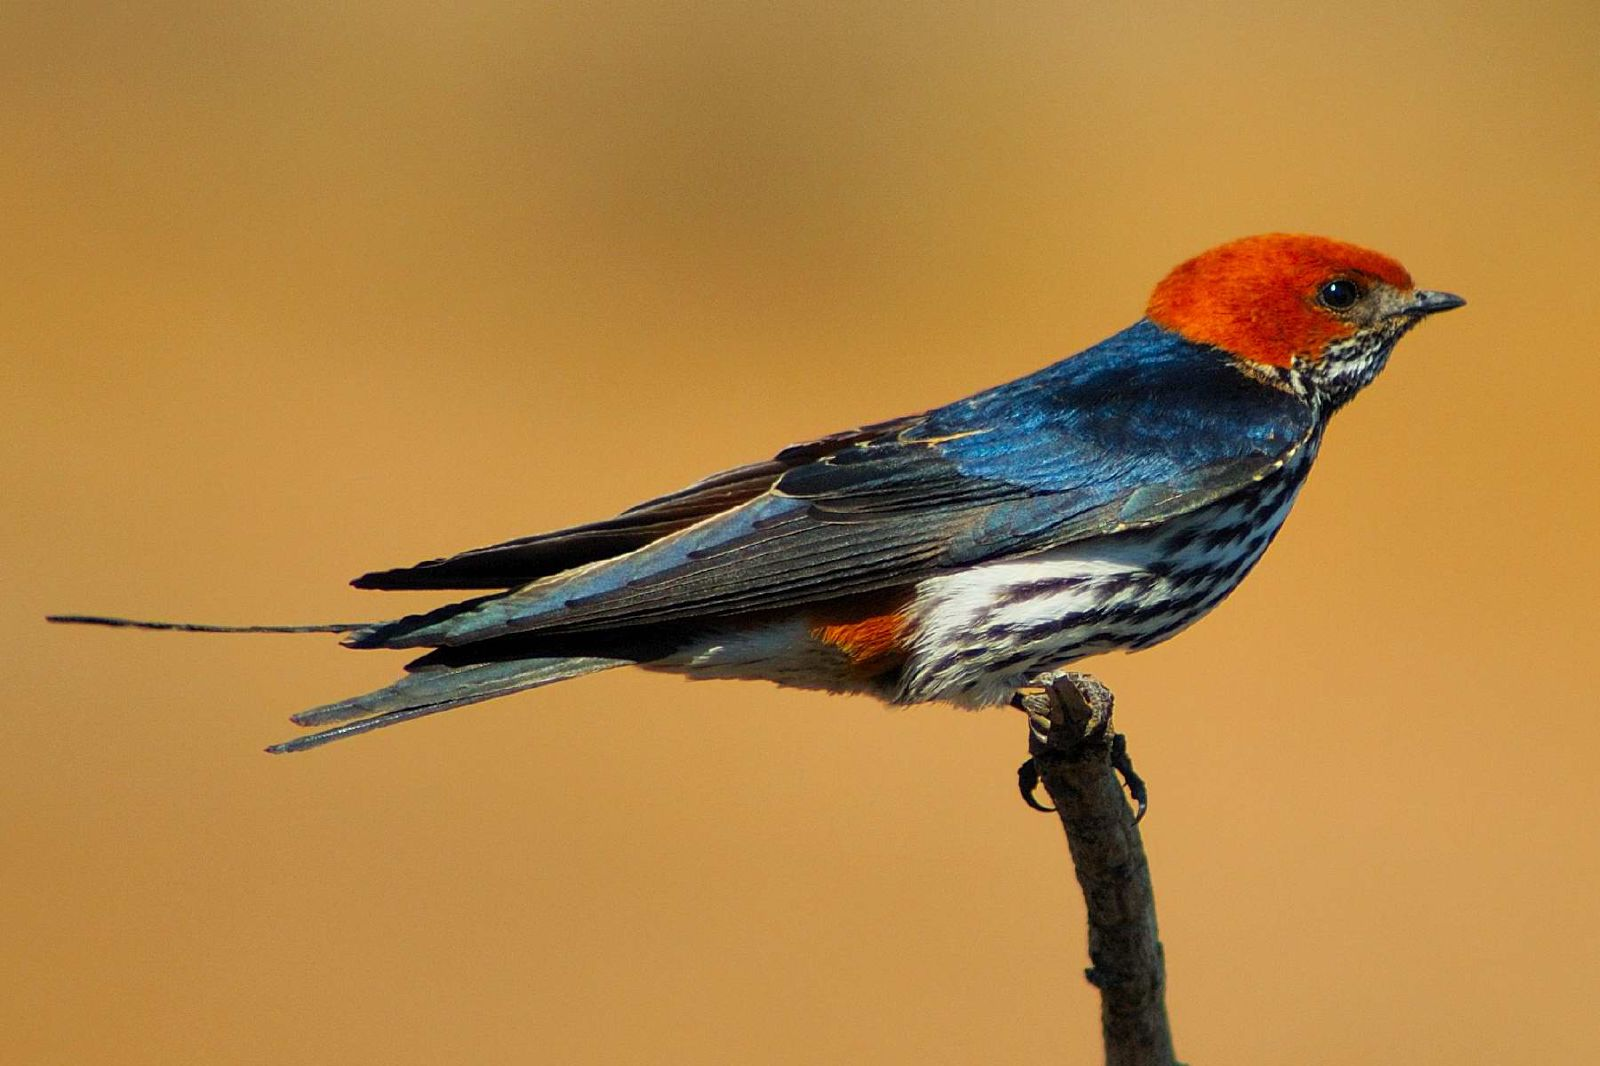
\includegraphics[width=0.6\textwidth]{Figures/swallow.jpg}
\caption{Training, validation and test loss of the neural network on the uniaxial compression/extension dataset.}
\label{fig:train_loss}
\end{figure}

\subsection{Comparison with Theoretical Curve and }
To further evaluate the accuracy of our neural network, we compared its predictions to the analytic solution for an input point outside of the training set. The conditions chosen for this comparison were $L_x = 1$, $p = 1$, and $E = 1$. The expected displacement of the center point of the prism's face is $u = 0.1667$, and the neural network predicted $u = 0.1667$, which amounts to an error of 0.0001. This is a very small error, indicating that the neural network is able to accurately predict the displacement of the center point of the prism's face.
\subsection{Evaluation on Cantilever Model}
For the case of the composed cantilever model, the training, validation and test loss is shown in Figure \ref{fig:composed_cantilever_loss}. As we can see, the training loss decreases rapidly during the first few epochs and then levels off. The final training loss is xxxx, indicating that the network has learned the underlying mechanical problem well.

\begin{figure}[h]
\centering
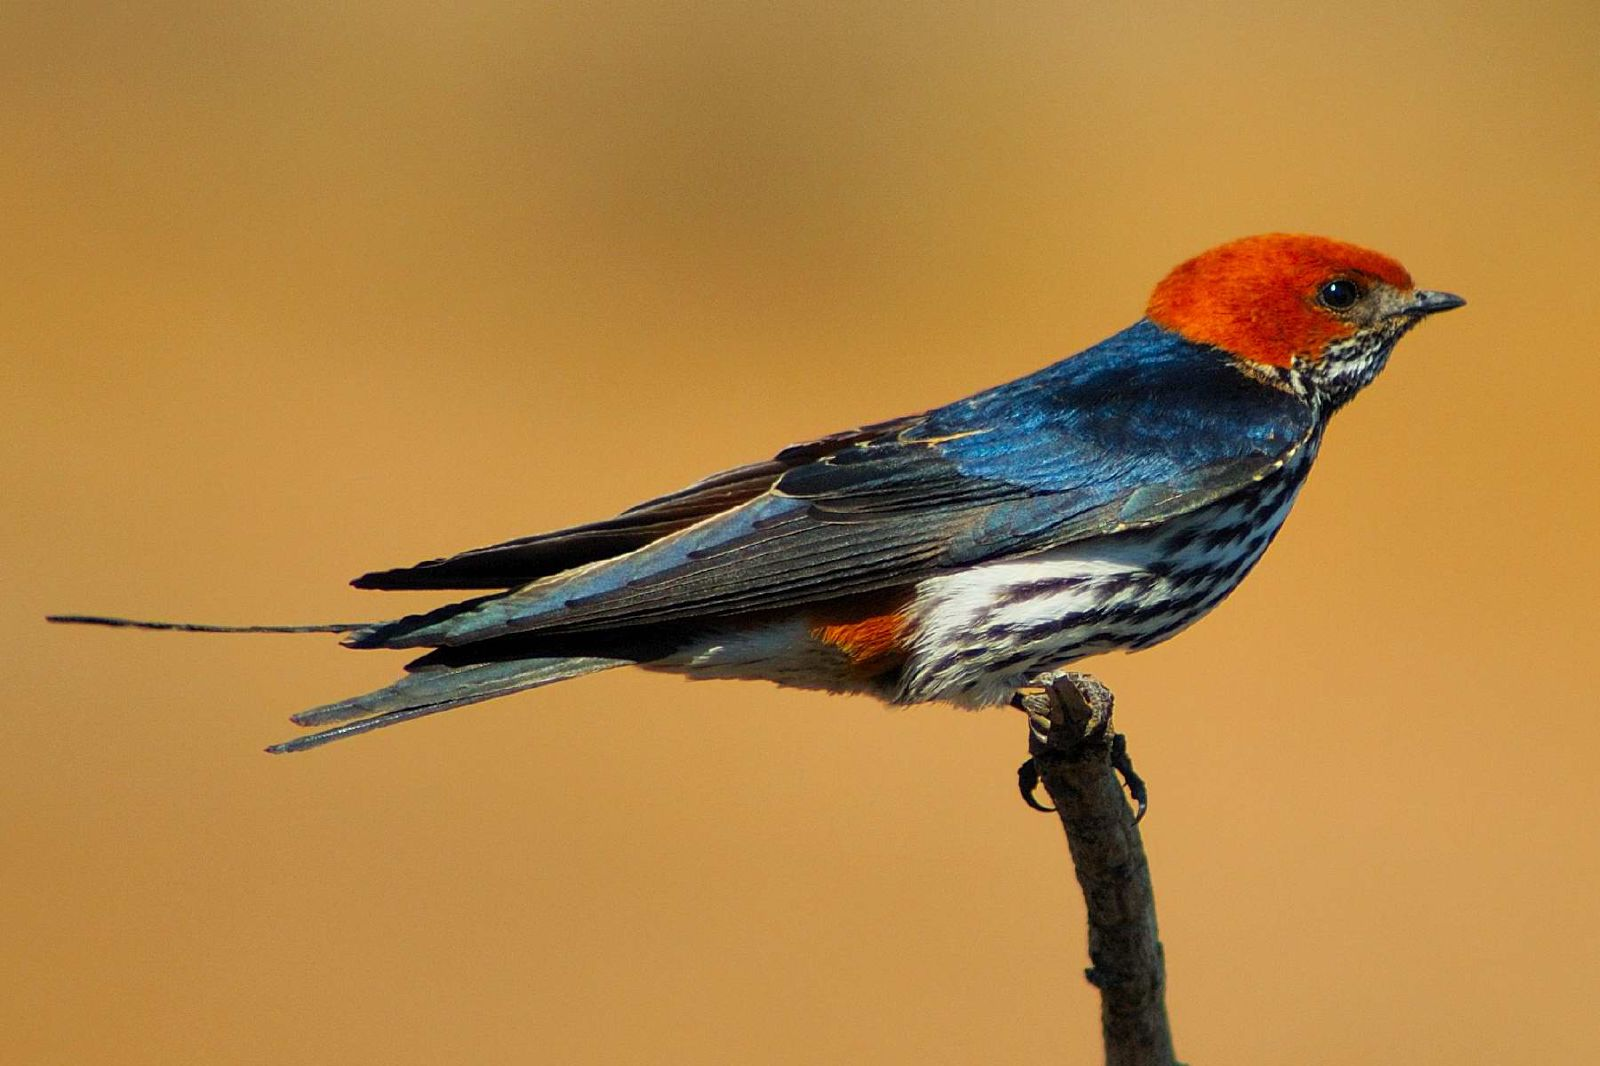
\includegraphics[width=0.6\textwidth]{Figures/swallow.jpg}
\caption{Training, validation and test loss of the neural network on the composed cantilever dataset.}
\label{fig:composed_cantilever_loss}
\end{figure}

\section{Conclusion}
In this project, we developed a pipeline for generating a dataset of FEM solutions to unidimensional compression/extension problems, and used this dataset to train a neural network to solve the same mechanical problem more quickly. Our experiments showed that our approach was effective, with the neural network achieving low losses on both the training and test datasets, and closely matching the theoretical curve for uniaxial compression/extension. We also demonstrated that our approach has the potential to be extended to more complex mechanical problems, as shown by our evaluation on a cantilever model. Overall, this project has the potential to significantly improve the efficiency of solving unidimensional mechanical problems, with broader implications for the engineering design process.

One advantage of our approach is its simplicity. By using a relatively simple unidimensional mechanical problem, we were able to develop a pipeline that can be easily scaled to more complex problems. Additionally, the use of a neural network allows for faster computation times than the traditional FEM method. This has the potential to significantly reduce computational costs for engineering design processes that rely on FEM simulations.

In conclusion, this project demonstrates the effectiveness of using a neural network to solve unidimensional mechanical problems. By developing a faster surrogate model, we have shown the potential to significantly improve the efficiency of solving such problems, with broader implications for the engineering design process. Future work includes scaling our approach to more complex mechanical problems and evaluating its effectiveness on a larger dataset.

\end{document}
